\documentclass[]{spie}  %>>> use for US letter paper
%\documentclass[a4paper]{spie}  %>>> use this instead for A4 paper
%\documentclass[nocompress]{spie}  %>>> to avoid compression of citations

\renewcommand{\baselinestretch}{1.0} % Change to 1.65 for double spacing

\usepackage{amsmath,amsfonts,amssymb}
\usepackage{graphicx}
\usepackage[colorlinks=true, allcolors=blue]{hyperref}
\usepackage{float}
%\usepackage{natbib}

\usepackage[textsize=tiny,textwidth=0.72in]{todonotes}
\usepackage{soul}
\usepackage{color} % color added for editing
\newcommand{\bl}[1]{\textcolor[rgb]{0.00,0.00,1.00}{#1}}
\newcommand{\gr}[1]{\textcolor[rgb]{0.00,0.50,0.00}{#1}}
\newcommand{\rd}[1]{\textcolor[rgb]{0.75,0.00,0.00}{#1}}
\newcommand{\tl}[1]{\textcolor[rgb]{0,0.6,0.60}{#1}}

\title{A compensation technique for accurate acceleration measurements using a UAV deployable and retrievable sensor package}

\author[a]{Joud Satme}
\author[a,b]{Austin R.J. Downey}
\author[c]{Jason D. Bakos}
\author[a]{Nikolaos Vitzilaios}
\author[b]{Dimitris Rizos}
\affil[a]{Department of Mechanical Engineering, University of South Carolina, Columbia, SC, USA 29201 }
\affil[b]{Department of Civil and Enviomental Engineering, University of South Carolina, Columbia, SC, USA 29201}
\affil[c]{Department of Computer Science and Engineering, University of South Carolina, Columbia, SC, USA 29201}


\authorinfo{Further author information: (Send correspondence to Joud Satme)\\Joud Satme: E-mail: Jsatme@sc.edu}

% Option to view page numbers
\pagestyle{empty} % change to \pagestyle{plain} for page numbers   
\setcounter{page}{301} % Set start page numbering at e.g. 301

\begin{document} 
	\maketitle
	
	\begin{abstract}
				
		The rapid assessment of infrastructure following extreme weather or seismic events is important to ensure stability of structures before continued use. This work presents an amplitude compensation technique for accurate acceleration measurements formulated for unoccupied aerial vehicle (UAV) deliverable sensor packages. These packages are designed for measuring the acceleration of structures, for instance, railroad bridges and power transmission towers. Current technology for structural health monitoring is expensive, stationary, and requires maintenance by certified personnel. These attributes prevent rapid assessment of remote and hard-to-reach structures. Low-cost, UAV-delivered sensor packages are an ideal solution due to their ability to be deployed on a large scale in a timely manner; cutting down on cost and the danger affiliated with structural health monitoring following extreme and hazardous events. One challenge to this approach is that the UAV deployable sensor package consists of a number of systems, including mounting hardware, embedded electronics, and energy storage that result in a loss of transmissibility between the structure and the package’s accelerometer. This work proposes a frequency response-based filter to isolate the structure’s vibration signature from interference caused by the sensor package itself. Utilizing an input-output relationship between the sensor package and a calibrated reference accelerometer, a model transfer function is constructed. Compensation is performed in the post processing stage using the inverse transfer function model. This approach is shown to enhance the signal-to-noise ratio by 1.2 dB, an increase of 7.17\%. This work investigates algorithm robustness and sensitivity to noise across the sensor package's bandwidth of 6-20 Hz. A discussion on the limitations of the system is provided.  
	\end{abstract}
	
	% Include a list of keywords after the abstract 
	\keywords{Accurate acceleration measurements, UAV deployable sensor, Transfer function-based filter, Signal-to-Noise ratio compensation, sensor node}
	
	\section{INTRODUCTION}
	\label{sec:intro}  % \label{} allows reference to this section
	
	In structural health monitoring, current systems operate as a mounted cluster of sensors permanently fixed onto and around the structure in question \cite{Pakzad2008}. These systems are typically installed later by specialists with dedicated instruments and vehicles as they are rarely considered during the structure's construction. This procedure is very time consuming and cost ineffective, as the sensing systems can’t be removed when not in use and their maintenance is as complex as the installation process. While traditional manual methods for sensor deployments have certain advantages, their use is limited in structures where deployments can be complex, remote locations where access to specialized vehicles for deployment is limited, or in safety-critical situations that limit options for human interaction with the structure. 

	The UAV-deployable sensor system considered in this work is a low-cost micro electromechanical system (MEMS) alternative \cite{Sabato2017} that is independently powered and compact enough to be aerially deployed to remote test sites, otherwise inaccessible by conventional methods. UAV deployment of an early-stage prototype package was demonstrated by Carroll et al. \cite{Carroll2021}. Utilizing an electropermanent magnet, the sensor packages can be mounted onto any metal surface on the structure being tested with minimal evasive effects \cite{Takeuchi2017} and can withstand long deployment periods due to the independent power system onboard. This system monitors the power consumption while conserving energy by turning off non vital parts of the sensor package when not in use. The package uses additional sensors to measure environmental parameters along with the vibration signature of the structure being inspected. Data is stored in onboard memory while a wireless system is used for data retrieval on demand. 

	This sensing system offers ease of use, high mobility, and low-cost. Important parameters for the deployment of wide-spread sensing networks in structural health monitoring applications. Rapid inspection can be made possible by deploying multiple packages that work in tandem to, more accurately, quantify damage from the vibration signature of the structure. With the aid of UAV system, the sensor packages can be placed in vital locations where damage is suspected to occur \cite{Chen2010}. Once deployed, the challenge becomes detecting the low-energy signals that are of interest when investigating damage. 

	
	In this work, a transfer function-based filter is proposed to enhance the signal to noise ratio (SNR\textsubscript{dB}) of the sensor package’s accelerometer. Using a known excitation signal and an input output relationship between two accelerometers a filter can be modeled to attenuate interference and transmissibility losses\cite{BADRI2010}. The filter designed in this work utilized a comparison between the micro electromechanical system (MEMS) accelerometer, onboard the deployable sensor package, and a reference lab-grade piezoelectric accelerometer. The comparison focus on the sensor package's sensitivity in the lower frequency range (6-20 Hz) as those frequencies are typically found in large structures\cite{KARPEL1997}. The contributions of this work are twofold. First, a transfer function-based filtering approach is formulated for use with UAV-deployable sensor packages, secondly,  the considered UAV-deployable sensor packages is validated against a reference accelerometer for the frequency range of DC to 20 Hz.
	


	
	
	\section{MATERIAL AND METHOD}

This section reports on the previously developed sensor package hardware, the data collection algorithm, and the complementary UAV deployment and retrieval system. Additionally, information on the mathematical formulation of the transmissibility filter along with its experimental procedure is also covered.

		\subsection{UAV deployable sensor package}

	\begin{figure} [H]
	\centering
	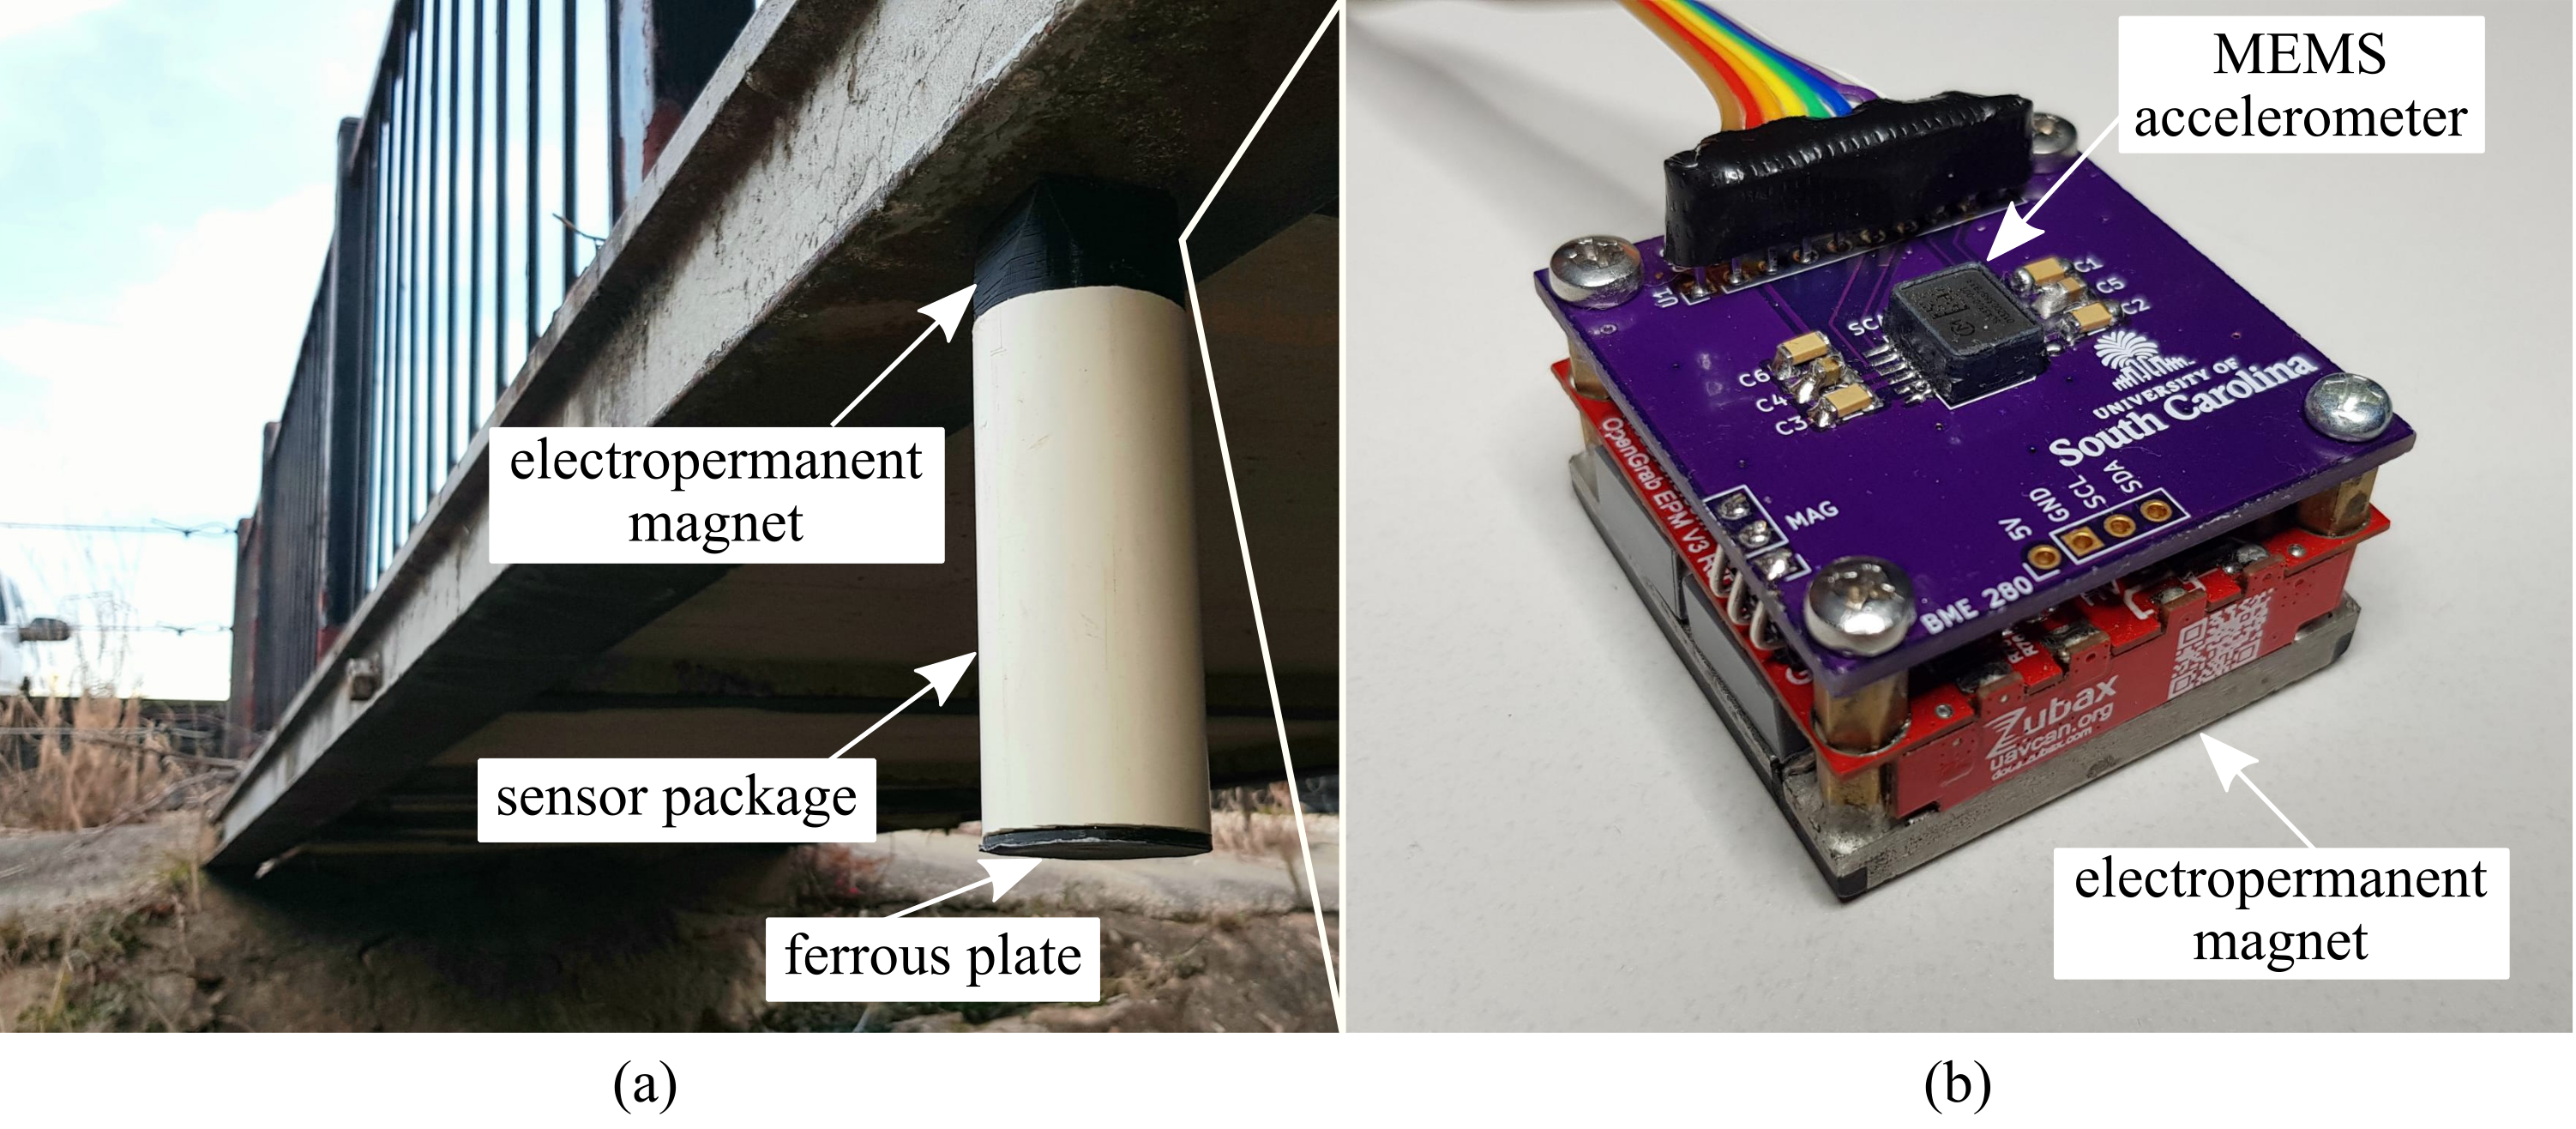
\includegraphics[width=6 in]{figures/MEMS.png}
	\caption{Micro electromechanical system (MEMS) accelerometer onboard the sensor package.}
	\label{fig:MEMS} 
	\end{figure} 	
	
The previously developed UAV deployable sensor package was designed with high mobility in mind as its weight and footprint had to be optimized for aerial delivery with payload limitations. Power and memory storage systems had to be incorporated into the design in anticipation for long deployment missions in remote areas where charging or unloading data off is not possible. A wireless subsystem along with data management and error handling algorithm was incorporated as well to enable the package to transmit data upon request from the user \cite{Sim2013}, gaining an advantage over wired systems.  With the main goal being vibration sensing, a sturdy contact with the structure was vital so a strong electropermanent magnet, with minimal power consumption was adopted. \bl{F}inally, the electronics and frame of the package where designed with minimizing transmissibility losses in mind because of the low-power ambient vibration signals to be measured. The data gathered using such system provides insight into structures' vibration signature and its natural frequencies, which caries information about the state of such structures\cite{Filippo2016}.  
	
	\begin{figure} [H]
		\centering
		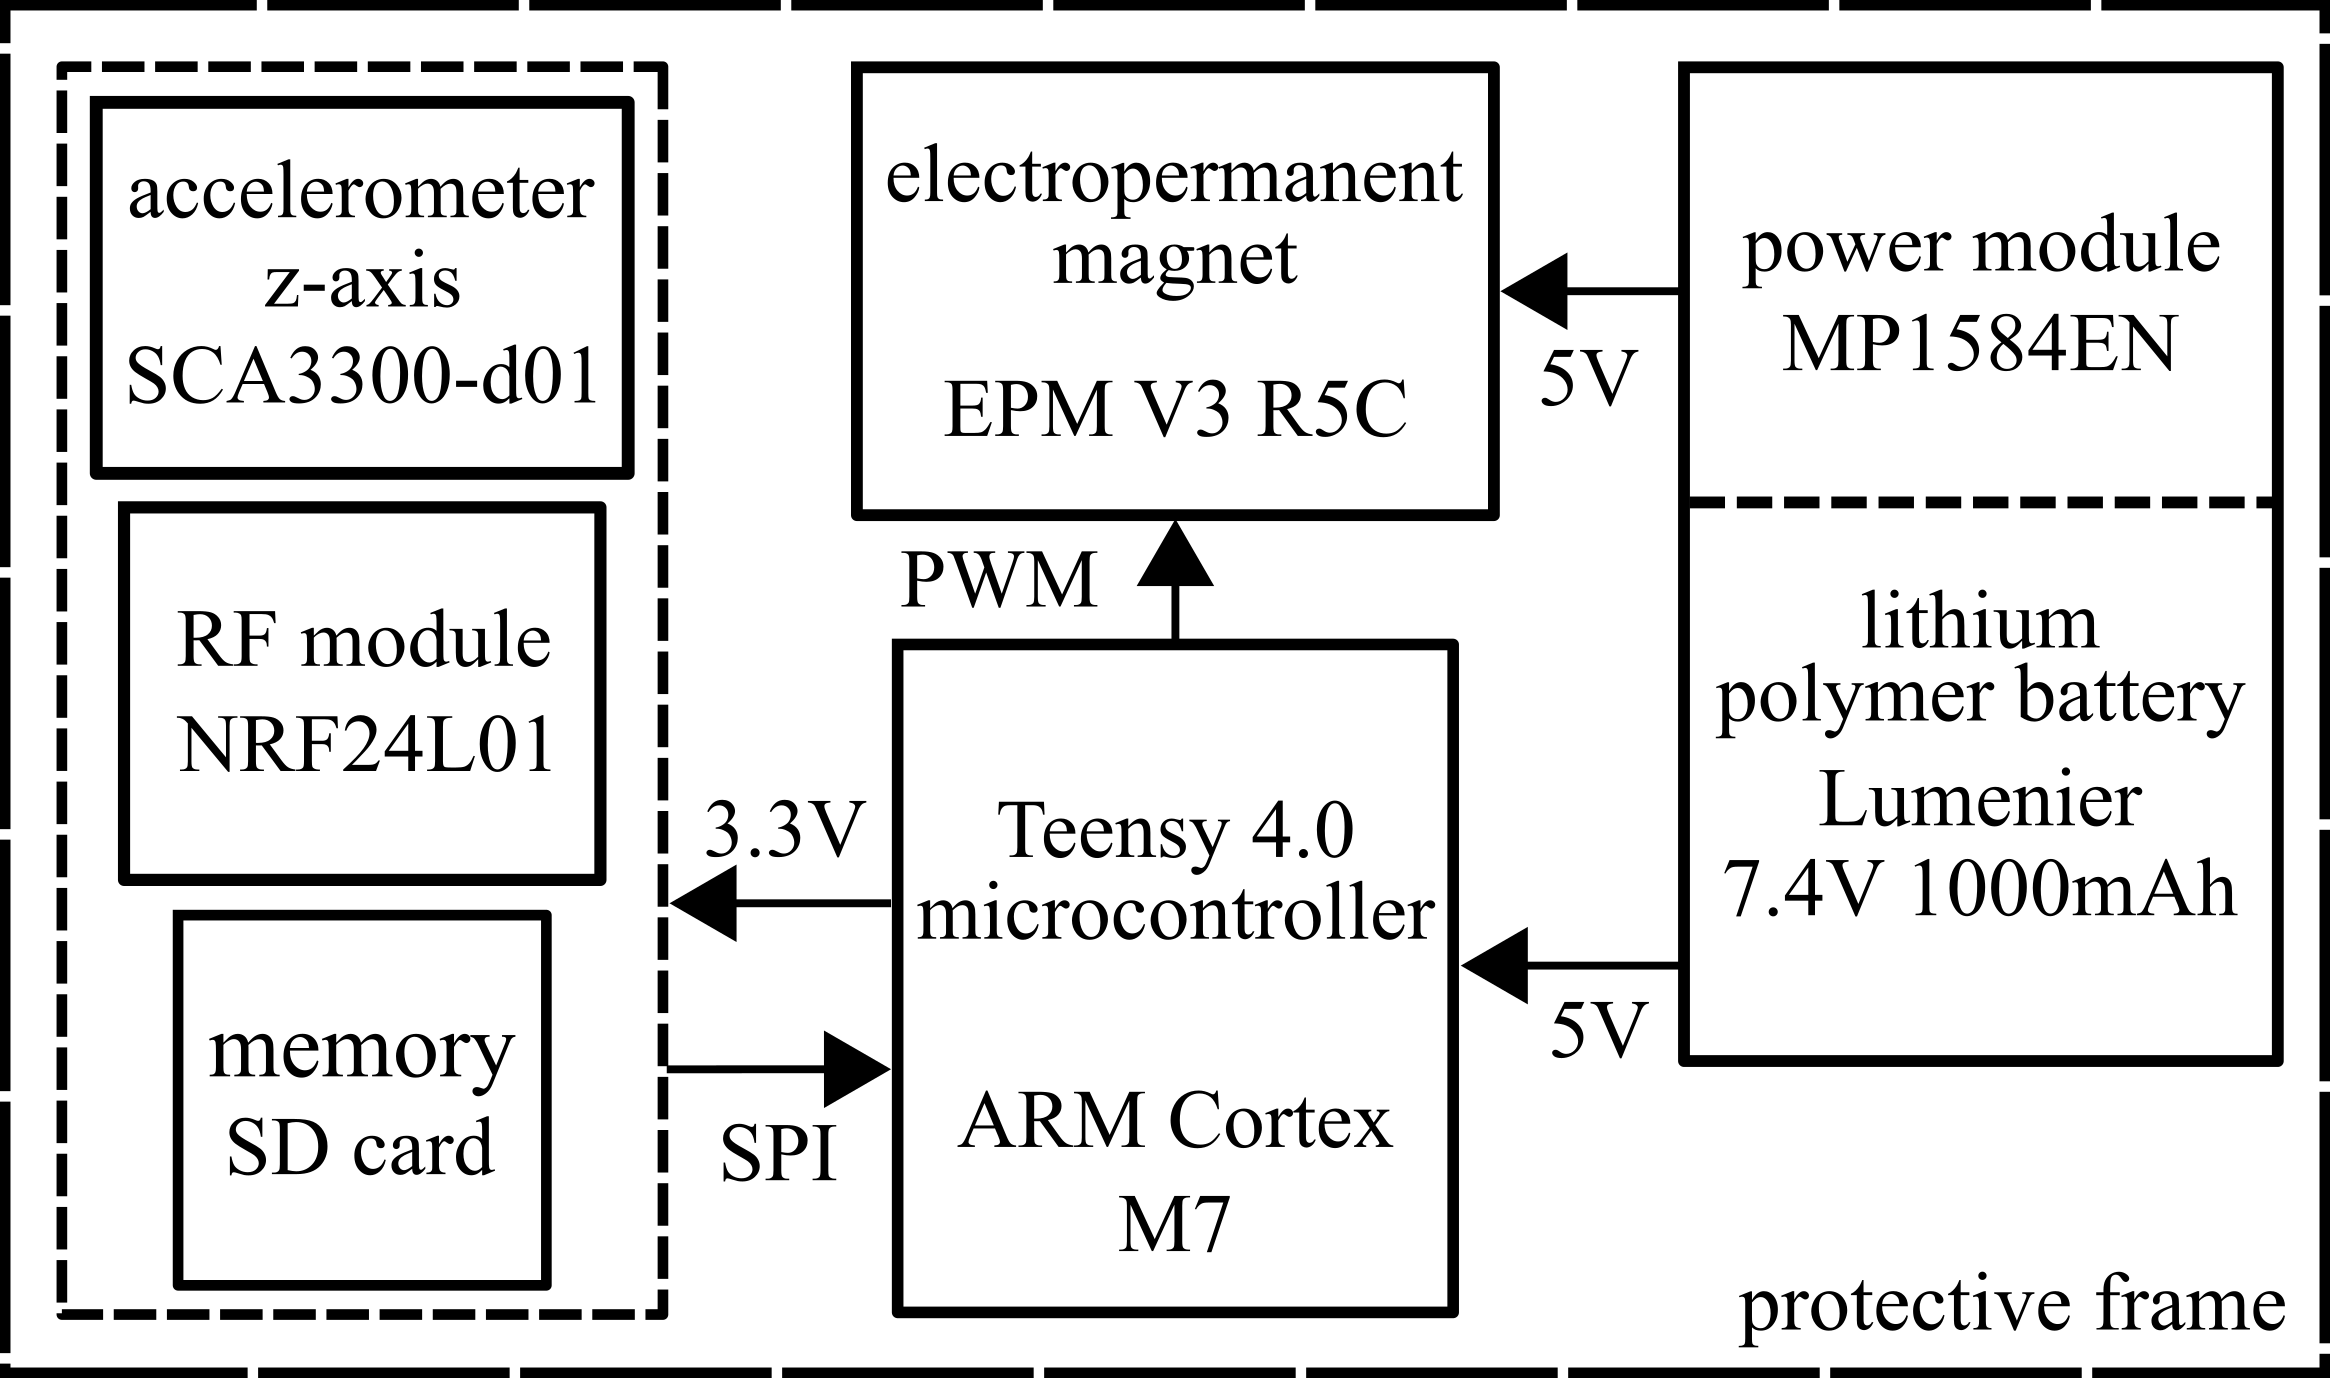
\includegraphics[width=4.66 in]{figures/SPIE Package Schematic.png}
		\caption{Block diagram depicting the various subsystems onboard the sensor package.}
		\label{fig:SPIE Package Schematic} 
	\end{figure} 	
	
	The sensor package's processor consists of the ARM Cortex-M7 onboard the Teensy 4.0. This high-performance microcontroller, with its 600 MHz clock and the serial peripheral interface (SPI) communication protocol, enables high-speed data collection up to 28 kS/s. As for the accelerometer used, a SCA3300-D01 MEMS accelerometer IC (manufactured by Murata) was mounted onto a custom PCB with its placement optimized to limit transmissibility losses. This PCB is directly fixed to the frame of the electropermanent magnet, which is assume to provide the best acceleration transmissibility from the structure, as shown in figure~\ref{fig:MEMS}(b). The electropermanent magnet (EPM V3R5C manufactured by NicaDrone) is used due to its low power consumption; only drawing significant power when switching states (1000 mA for 0.75-1.2 s). During data collection, a sample size of 74,000 samples is recorded temporarily onto the Teensy 4.0 buffer to then be transferred to nonvolatile memory (SD card) for long-term storage, a process that approximately takes 3.288 s. With packages being required to deploy for up to 1 week at a time, a power monitoring and control system was developed to periodically measure the onboard Lithium polymer battery voltage and turn off all parts of the system that are not in use. This aids in extending the battery life to the desired deployment period. The sensor package is fitted with a wireless transceiver (NRF24L01 by Nordic Semiconductor) which enables the sensor package to send stored data and package status (power and memory capacity) on demand and receive commands to disengage the magnet during retrieval. The System's hardware is then fitted into a 3D printed frame that fits into a standard 2 in PVC pipe to shield the delicate electronics from the elements during operation. Sensor package circuit with key components annotated is shown in figure~\ref{fig:Sensor_Package_labeled_componenets}. The code was developed on the Arduino integrated development environment which is compatible with the Teensy 4.0 microcontroller used.  

	\begin{figure} [H]
	\centering
	\includegraphics[width=6in]{figures/Sensor Package labeled componenets.png}
	\caption{Hardware components for the UAV-deployalbe sensor package removed from the protective frame.}
	\label{fig:Sensor_Package_labeled_componenets}
	\end{figure}

	
	With the goal being mass deployment in remote and hard to reach locations, a UAV system was developed to allow the user to approach the structure with ease without the need for highly trained personnel and heavy machinery. The drone used in this work incorporates a deployment harness which included a magnet  and guiding rails. This system further increases safety and ease of use as it guides the sensor package to the mount during retrieval. The on-board electropermanent magnet aids in securing the retrieved package in place before disengaging the package’s magnet and flying back to base as shown in figure~\ref{fig:UAV_deployment}\cite{Carroll2021}.

	\begin{figure} [H]
		\centering
		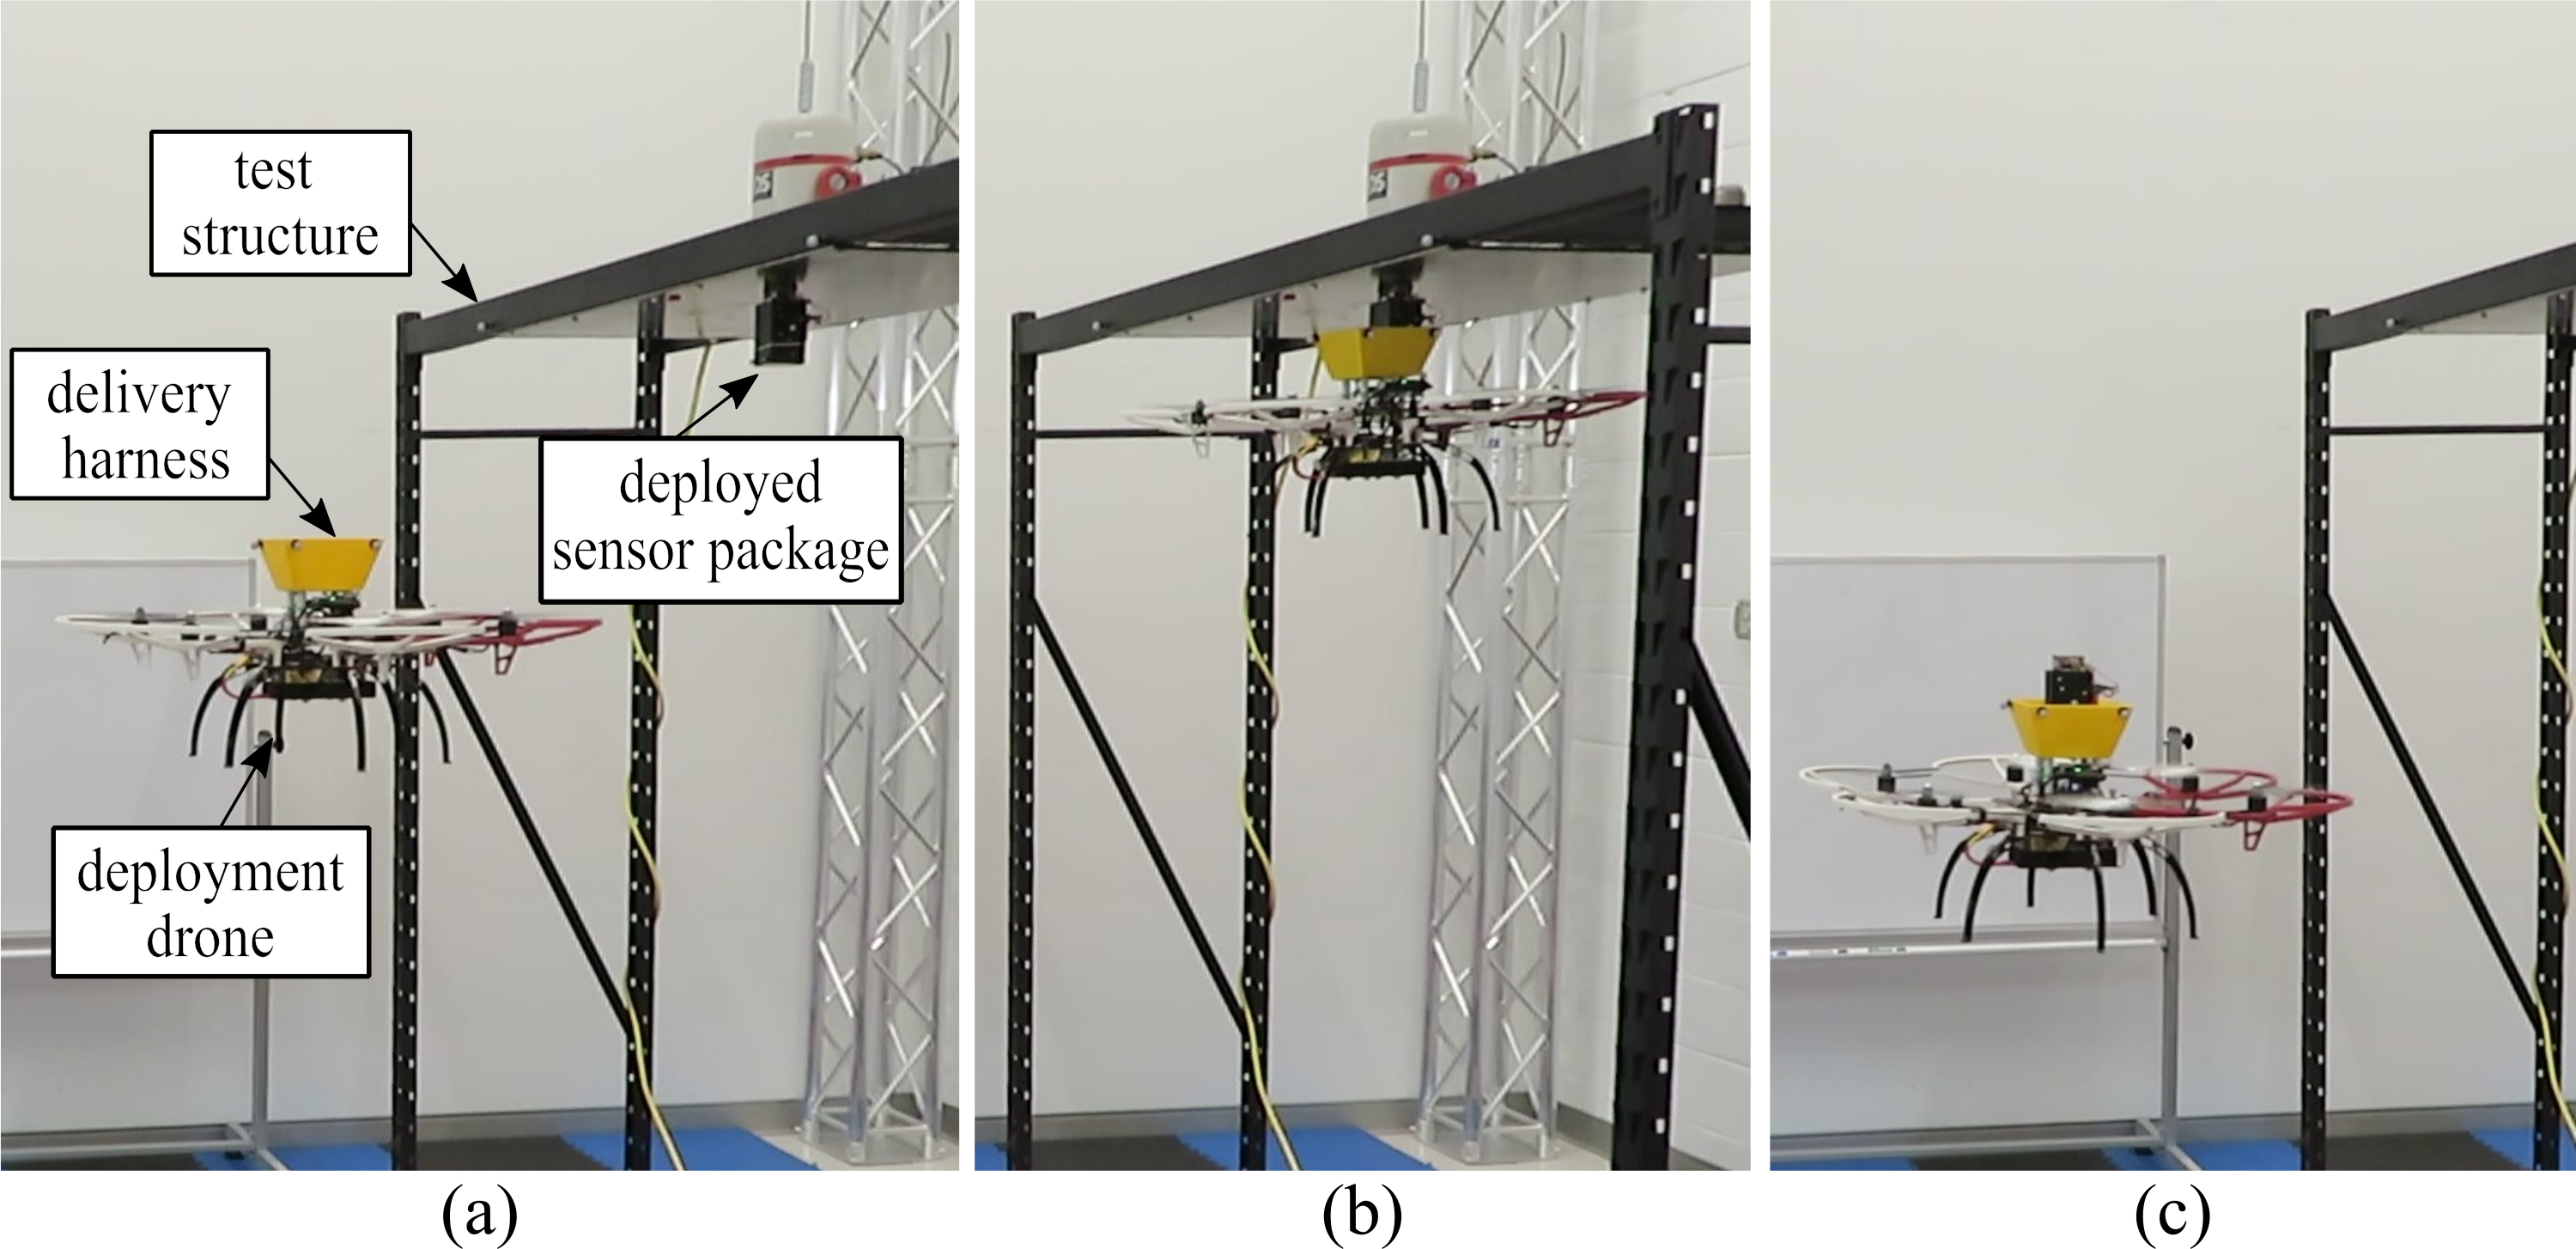
\includegraphics[width=6in]{figures/UAV deployment.png}
		\caption{Package retrieval mission depicted in three frames (a) UAV approach (b) UAV contact (c) successful retrieval.}
		\label{fig:UAV_deployment} 
	\end{figure}


	\begin{figure} [H]
		\centering
		
\includegraphics[height=17cm]{figures/Code FlowChart.png}
		\caption{Sensor package deployment mission code breakdown.}
		\label{fig:Code FlowChart} 
	\end{figure}
	


	During normal operation the code will start by initializing the magnet signaling the start of a deployment mission. Acceleration data is then periodically collected according to a preset schedule. Each set of data is first collected in the buffer to enable high sampling rates as vibration signature-based algorithms used in structural health monitoring require high time domain accuracy. After a maximum sample set of 64,000 samples is collected, the data is then transferred onto the SD card. The code then signals standby mode which turns all modules off but the microcontroller and the wireless module. Those two modules remain on in case communication with the package needs to be established. When communication is established, a user can request information about the operating conditions of the package, retrieve stored data, send IO commands to the magnet which signals the end of a deployment. A flow chart of the package’s code is shown in figure~\ref{fig:Code FlowChart}.
	
	\subsection{FILTER DESIGN}


	The sensor package's filter is developed through a transfer function-based approach. In this approach, an input output relation is acquired using various methods of excitation, such as frequency sweeps, impulse response, and white noise. Utilizing the input-output relationship, a model of the plant being studied can be created. Assumptions about the nature of the system have to be made during the modeling process. In this case, the system was considered to be a causal minimal phase system, $G$p$(s)$. When $G$p$(s)$ is inversed, a filter with the inverse characteristics of the plant’s frequency response is acquired. Using this filter, the influence of the plant is attenuated, with the true input obtained using only the output of $G$p$(s)$. The control scheme of the system is shown in figure~\ref{fig:Control_Scheme}.
	
	\begin{figure} [H]
		\centering
		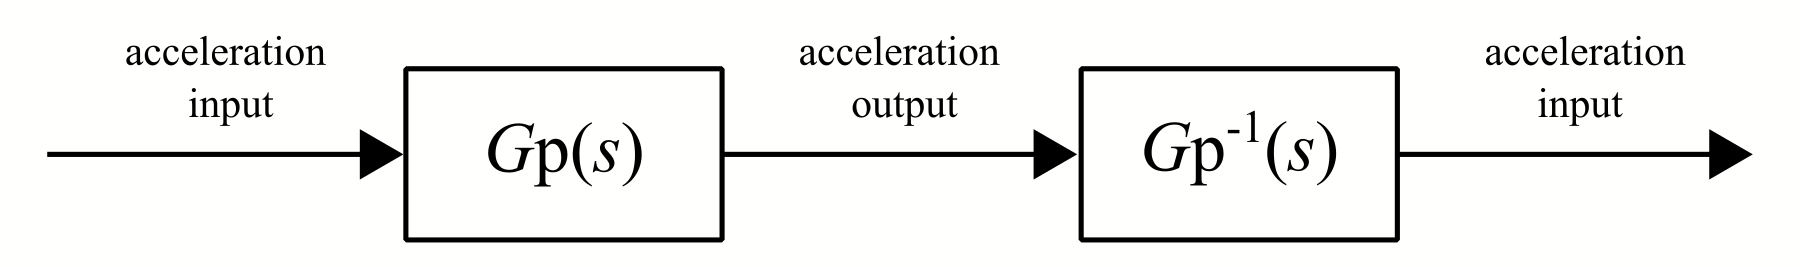
\includegraphics[width=6 in]{figures/Control Scheme.png}
		\caption{Control scheme of the inverse transfer function filter.}
		\label{fig:Control_Scheme}
	\end{figure} 


	In order to acquire the transmissibility transfer function $G$p$(s)$ of the sensor package’s frame, the sensor package is placed on an electromagnetic shaker along with a lab-grade accelerometer (model 393B04 from PCB Piezoelectric) to be used as reference. A chirp excitation was used to obtain the sensor package’s frequency response where the electromagnetic shaker was used to frequency sweep in the bandwidth of 6 to 20 Hz, the frequency range relevant in large structures. In this approach, the input-output relation of the reference accelerometer to the sensor package’s onboard accelerometer is recorded using a data acquisition system and then processed offline. The two sets of data are imported, synchronized, and interpolated to the same time scale. A model of the transmissibility of vibration through the sensor package is acquired with an acceptable level of correlation, the assumption that the inverse of the plant is stable when switching the zeros and poles’ location had to be made for this approach to be successful. When setting the model parameters, only the frequency components between 6 and 20 Hz were considered as this will further filter out the undesired high frequencies that may be present. The plant transfer function $G$p$(s)$ is then inversed; creating a filter transfer function $G$p$^{-1}(s)$. When the sensor package data is fed through the designed filter, unity gain is established, where the filter attenuates the influence of the sensor package’s frame on the acceleration that the onboard accelerometer registers. This enhances the sensor package’s signal to noise ratio reducing the transmissibility losses through the frame of the package. 
	
	\begin{figure} [H]
		\centering
		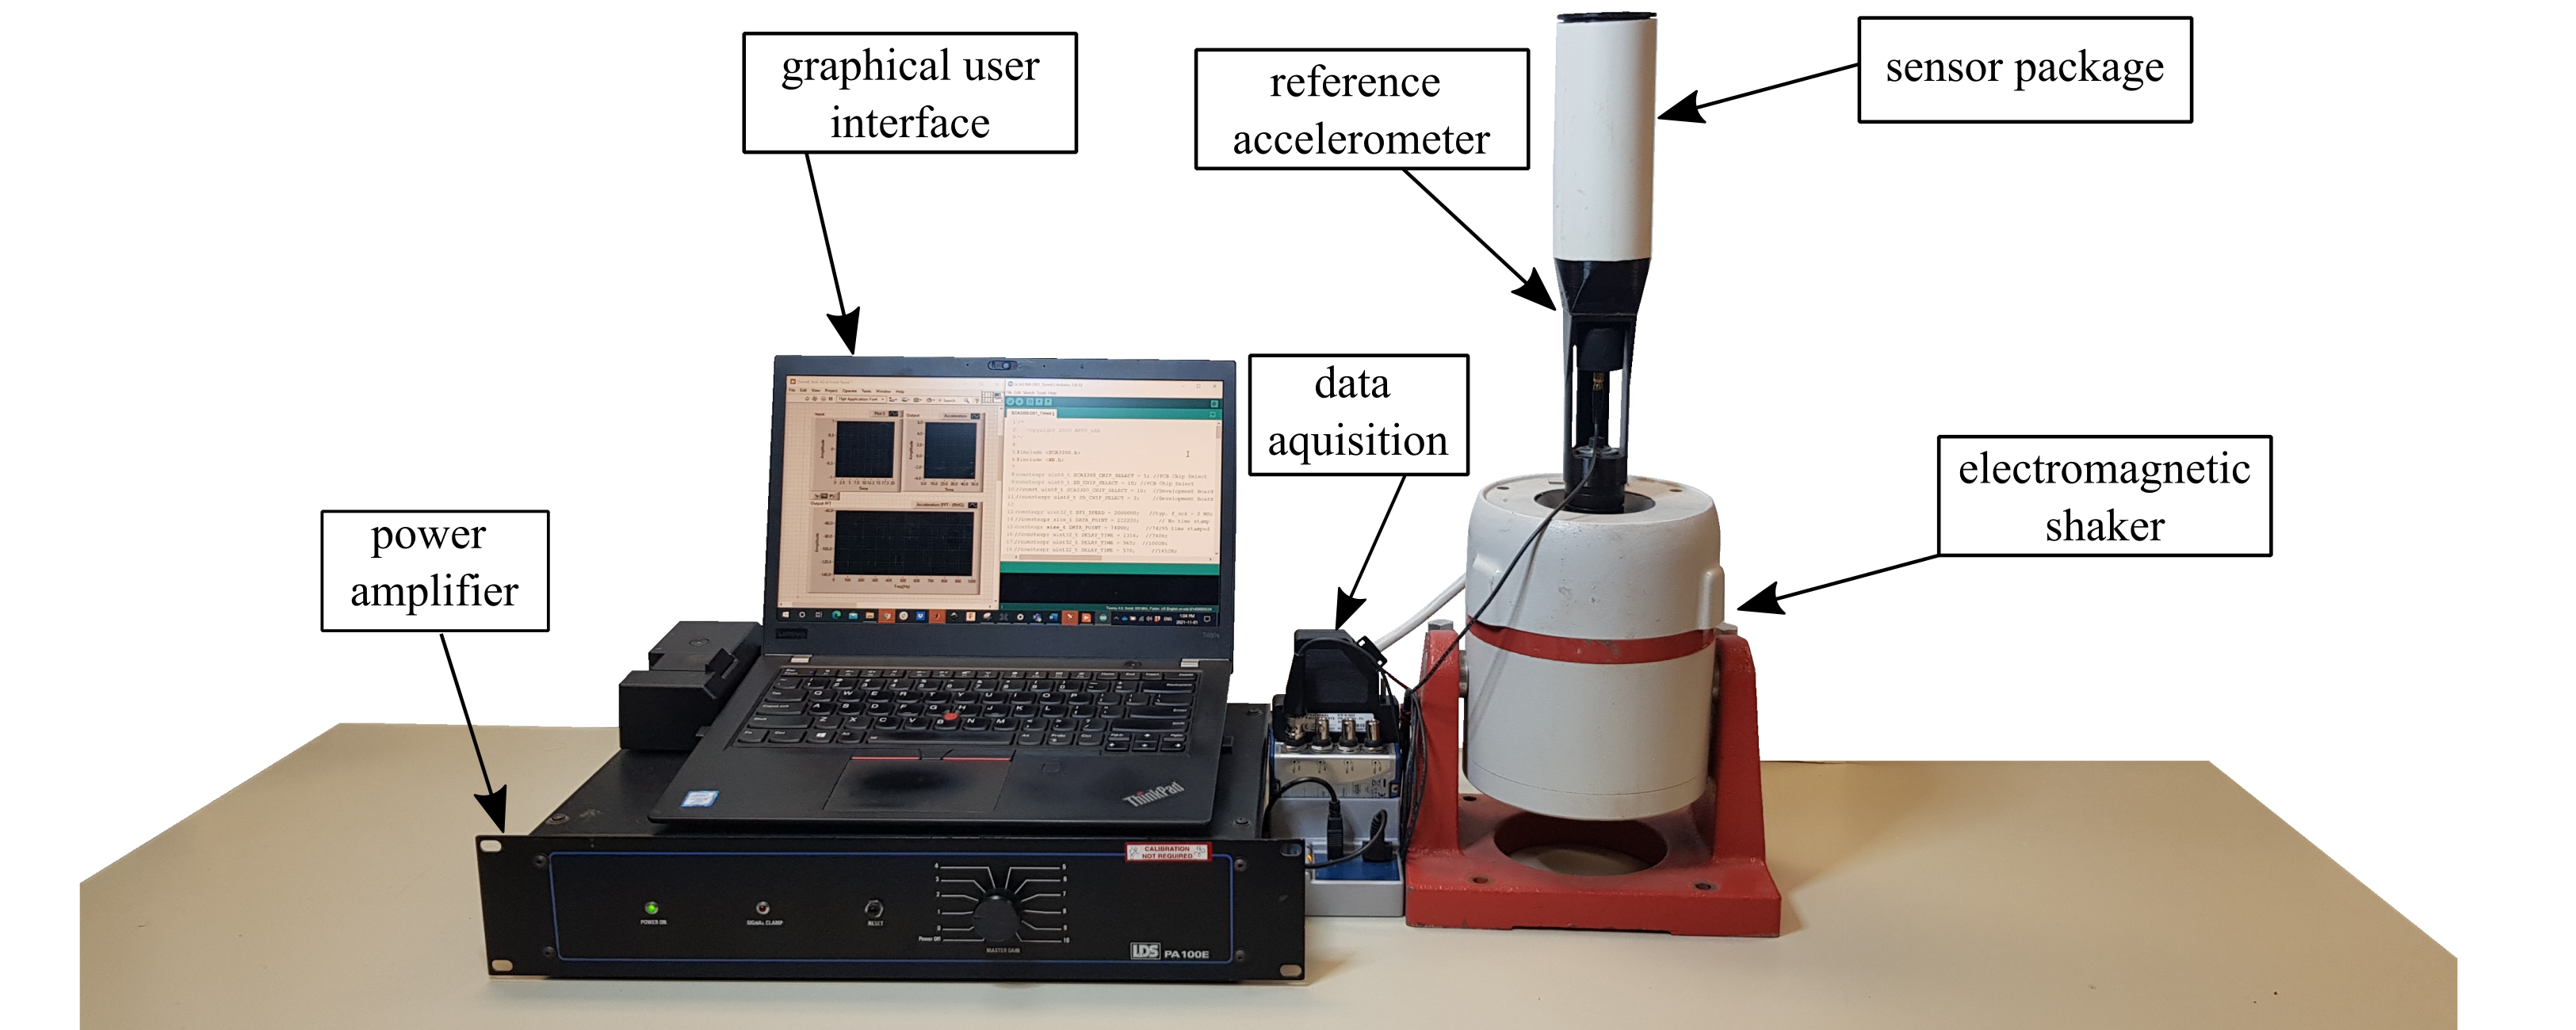
\includegraphics[width=6 in]{figures/benchtop_experimental_setup}
		\caption{Sesnor package frequency response experimental setup with labeled key components.} 
		\label{fig:bench top experimental setup}
		
	\end{figure} 

	
	Utilizing the experimental setup shown in figure~\ref{fig:bench top experimental setup}, any extra influence of a structure was eliminated as the focus of this experiment was to study the effect of the sensor package frame on the overall transmissibility of acceleration, from the immediate source (electromagnetic shaker) to the sensor package's onboard accelerometer. With the results of this experiment, an input-output relation was investigated to see where most transmissibility losses occur on the frequency spectrum. The Chirp approach chosen for the excitation signal made examining the bandwidth of DC to 20 Hz more feasible, as this type of excitation has a start and end frequency with no components beyond that window.
	
	\begin{figure} [H]
		\centering
		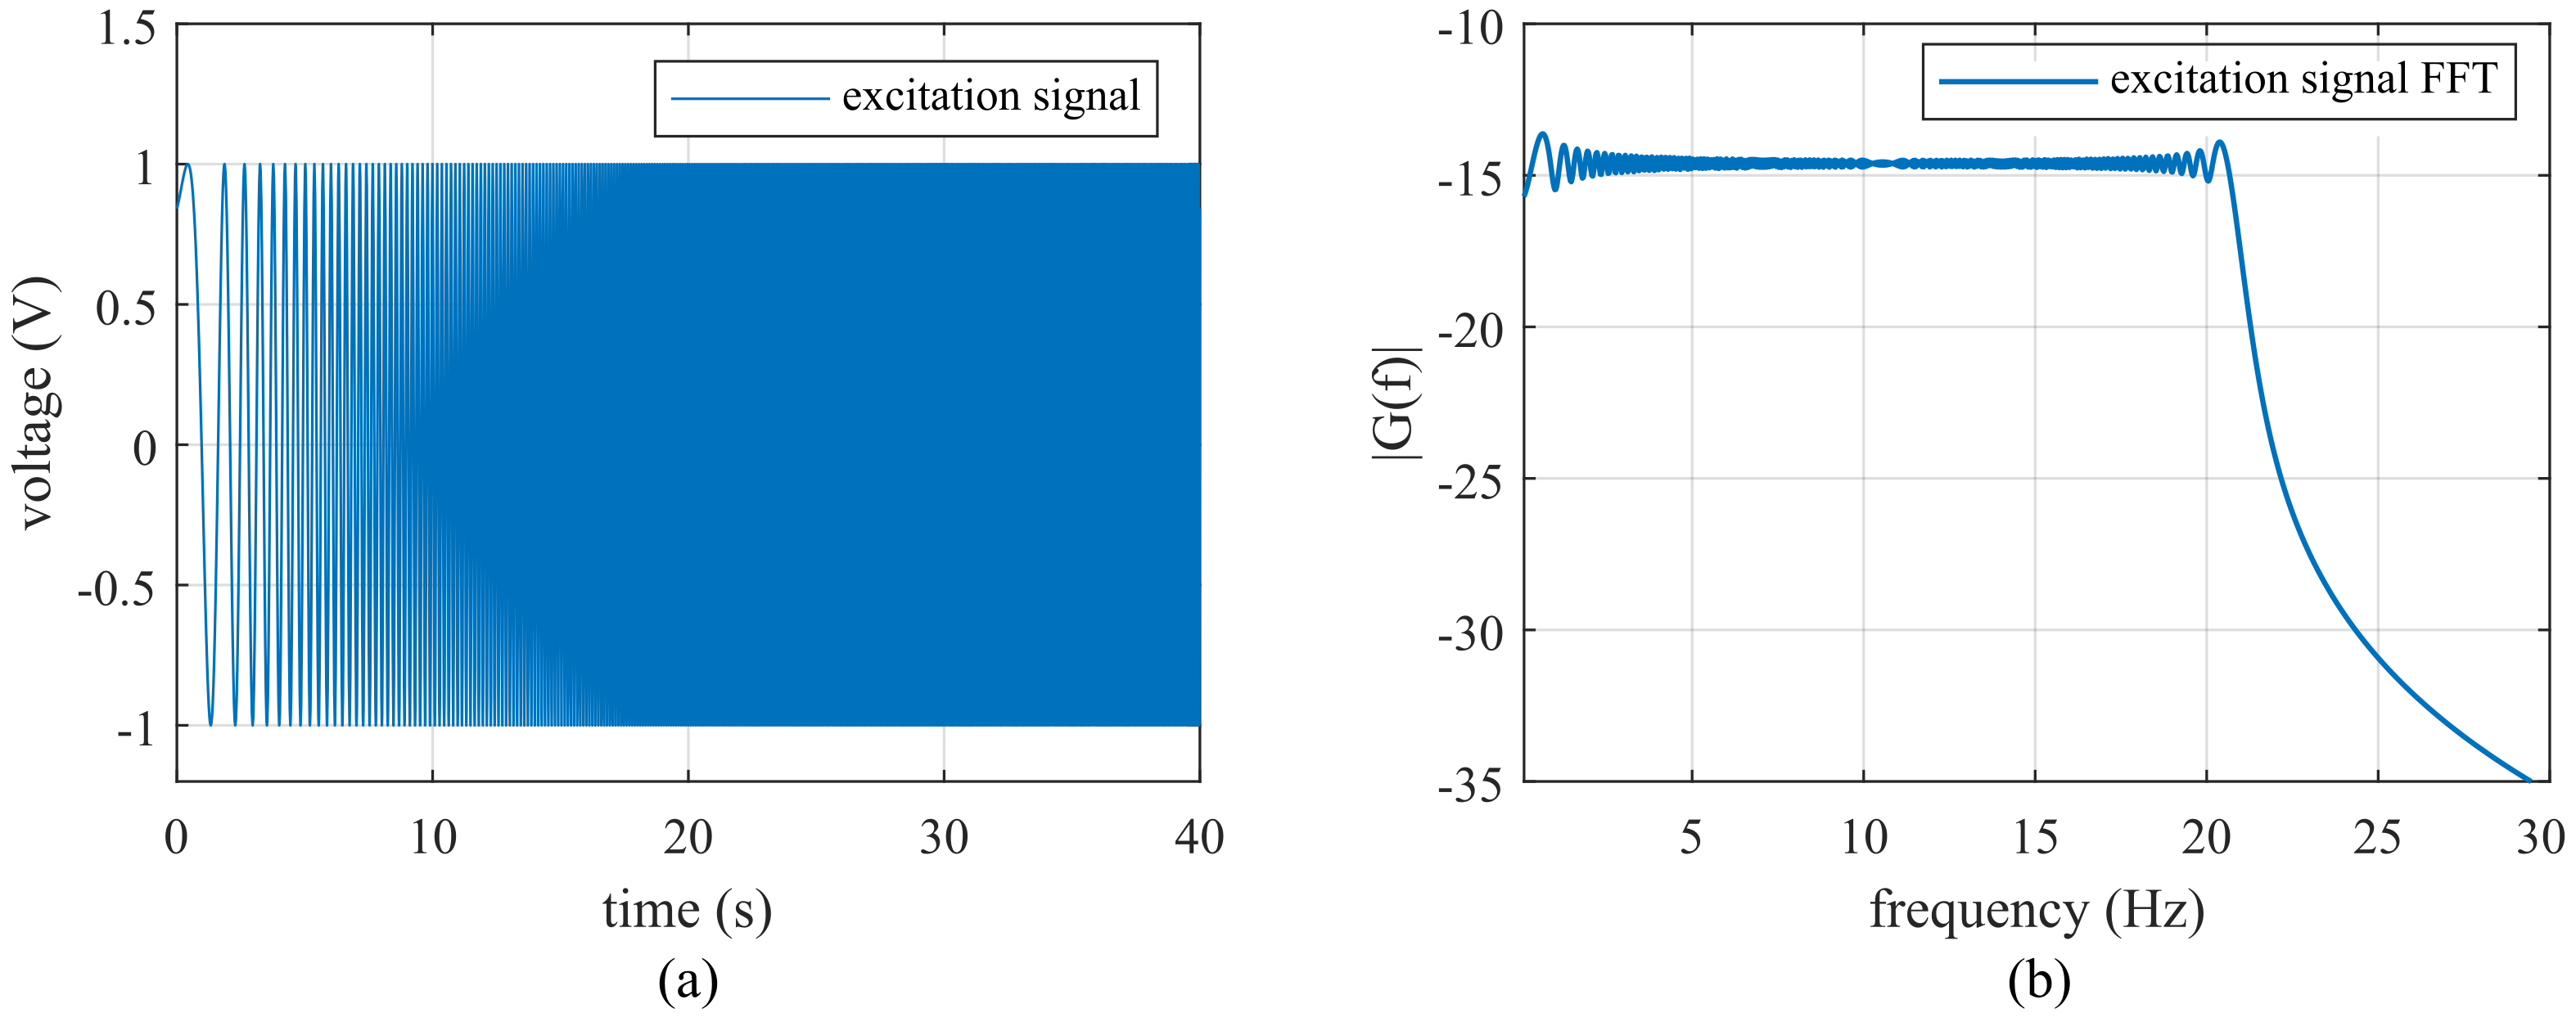
\includegraphics[width=6 in]{figures/excitation signal Time and Frequency domain chirp plot.png}
		\caption{Normalized chirp excitation signal: (a) time doamain; (b) frequency domain plots.} 
		\label{fig:excitation signal Time and Frequency domain chirp plot} 
	\end{figure}

	\begin{figure} [H]
		\centering
		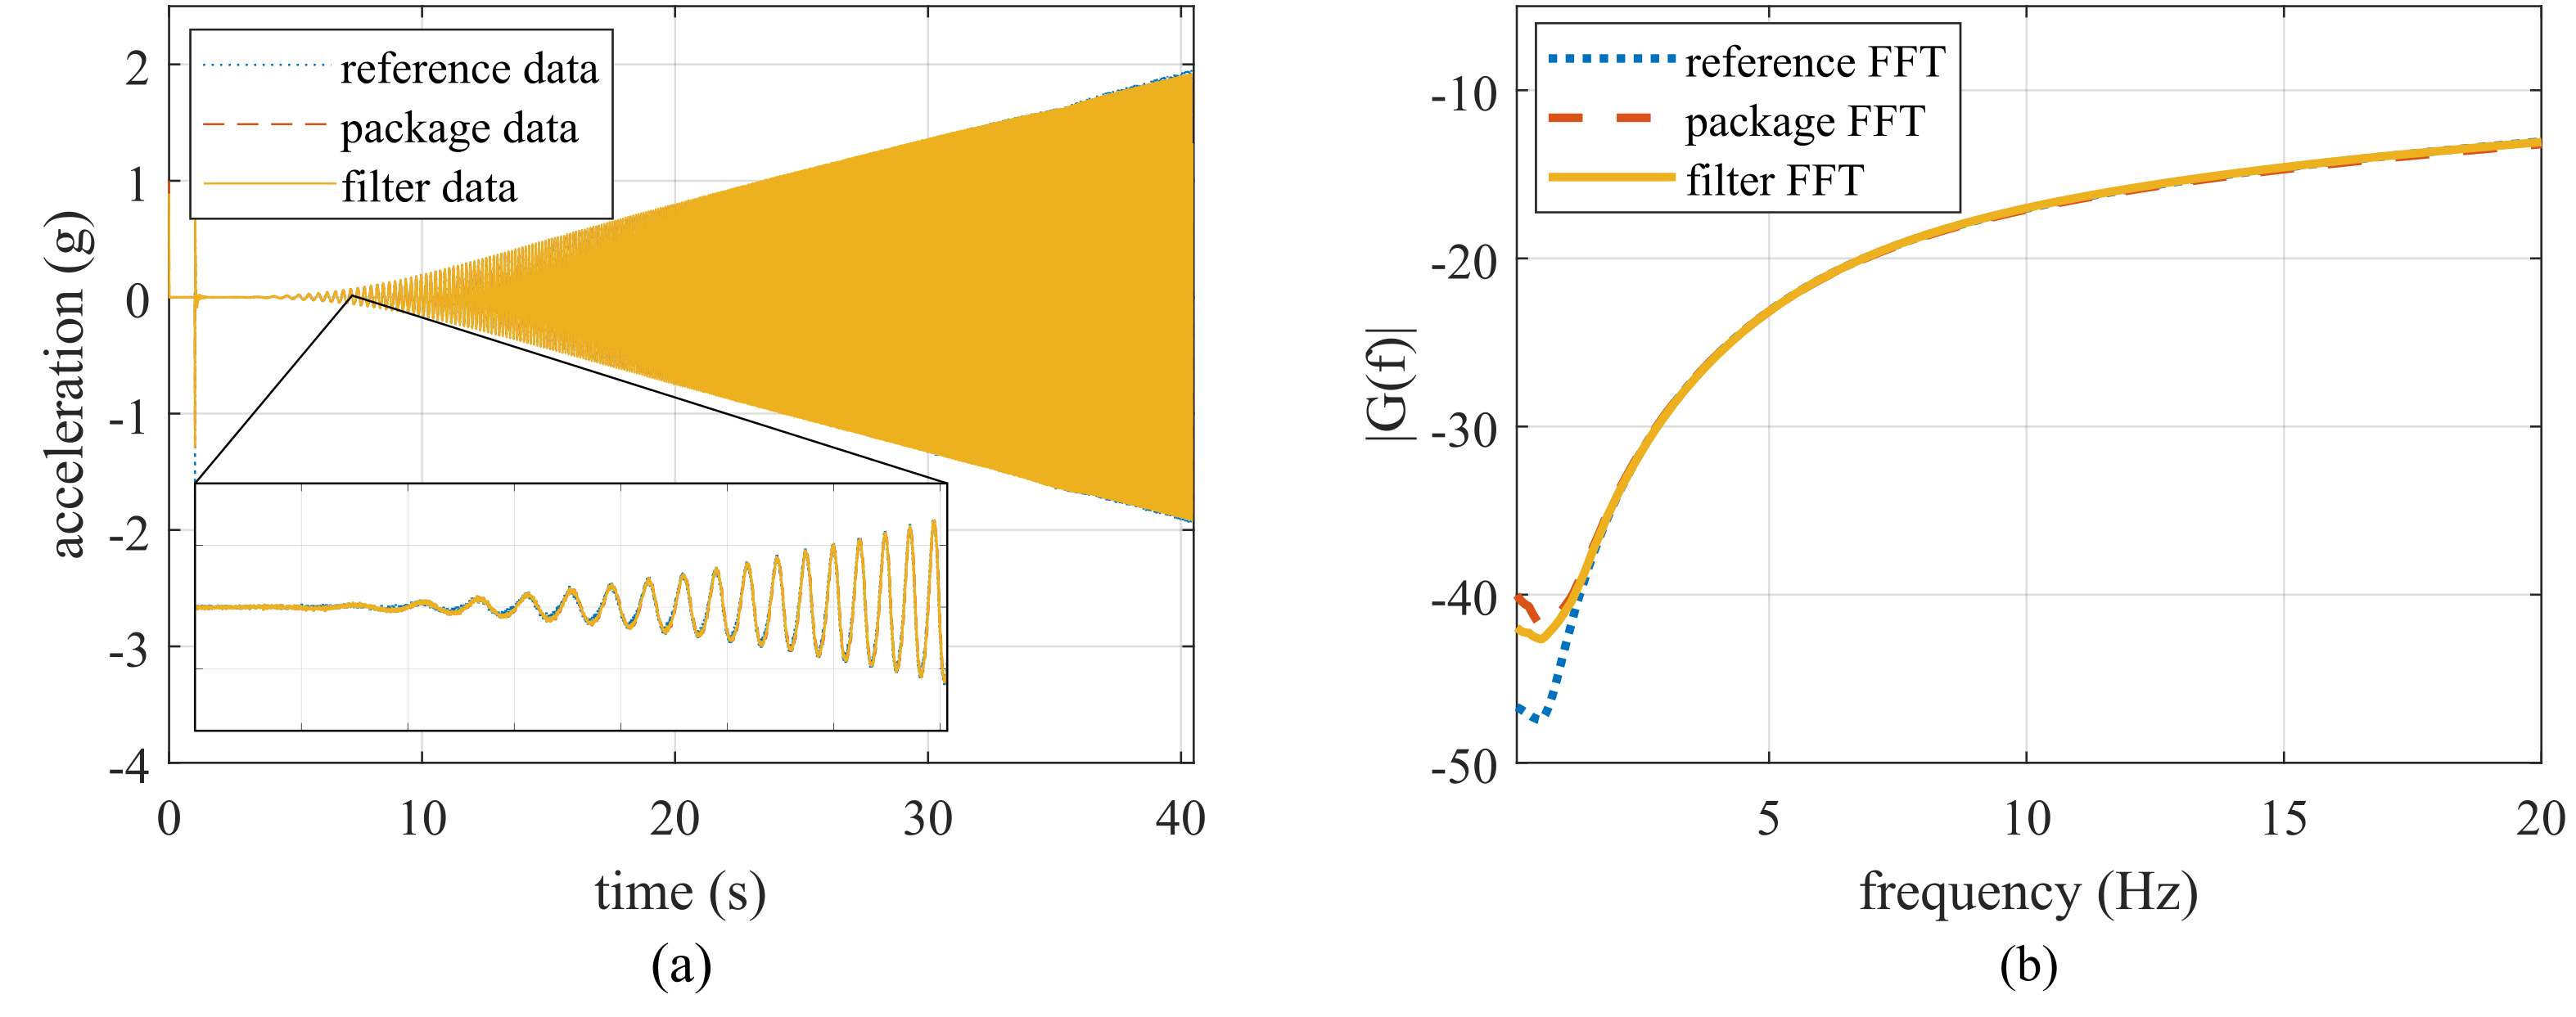
\includegraphics[width=6 in]{figures/Chirp Benchtop Filtered.png}
		\caption{Benchtop experiment comparison between pre and post filter performance in: (a) time domain; (b) frequency domain with respect to a reference accelerometer.} 
		\label{fig:excitation signal plot} 
	\end{figure}
	
	In this approach a chirp signal was constructed using equation~\ref{eq:Chirp}. Where $f_0$ is the initial frequency (0.1 Hz) and $f_1$ is the end frequency (21 Hz). $T$ was the length of the test, which lasted 40 s, dictated by the size of the buffer onboard the sensor package, which collects 40 seconds worth of data at a sample rate of 16,00 samples per second totaling 64,000 samples.
	
	\begin{equation} 
		\label{eq:Chirp}
		x(t)=\sin(1 + 2\pi ( \frac{(f_1-f_0)}{2T} ) t^2 + f_0 t) \, 
	\end{equation}
	

	
	Utilizing the chirp signal, the experiment was conducted and data from both the reference and package accelerometers were used in the modeling process. After interpolating the data and using the input output relation, a third order s-domain transfer function was constructed as shown in eq~\ref{eq:Gp}. 
	
	\begin{equation}
		\label{eq:Gp}
		G_\text{p}(s) = \frac{s^3  + 668.8 s^2  + 2.937e4 s + 3.58e4}{1.123 s^3  + 652.1 s^2  + 3.067e4 s + 7.393e4} \, 
	\end{equation}

To accurately evaluate the performance of the constructed filter, the signal-to-noise ratio, in decibels, was adopted as a metric. $\text{SNR}_{\text{dB}}$ was utilized to compare the condition of the measured acceleration signal, prior and post filtering, to gauge the noise rejection capabilities of the filter. $\text{SNR}_{\text{dB}}$ was calculated as the ratio of the summed squared magnitude of the measured signal S($i$) to the summed squared magnitude of the noise N($i$) taken on a log scale as shown in equation~\ref{eq:SNR}.~\cite{Johnson2006}

%\begin{center}
	\begin{equation}
		\label{eq:SNR}
		\text{SNR}_{\text{dB}} =10 \log_{10}(\frac{\Sigma^{74000}_{i=1}(S(i))^2}{\Sigma^{74000}_{i=1}(N(i))^2}) \, 
	\end{equation}
%\end{center}

	
	\section{TESTING AND VALIDATION}
	


	\begin{figure} [H]
		\centering
		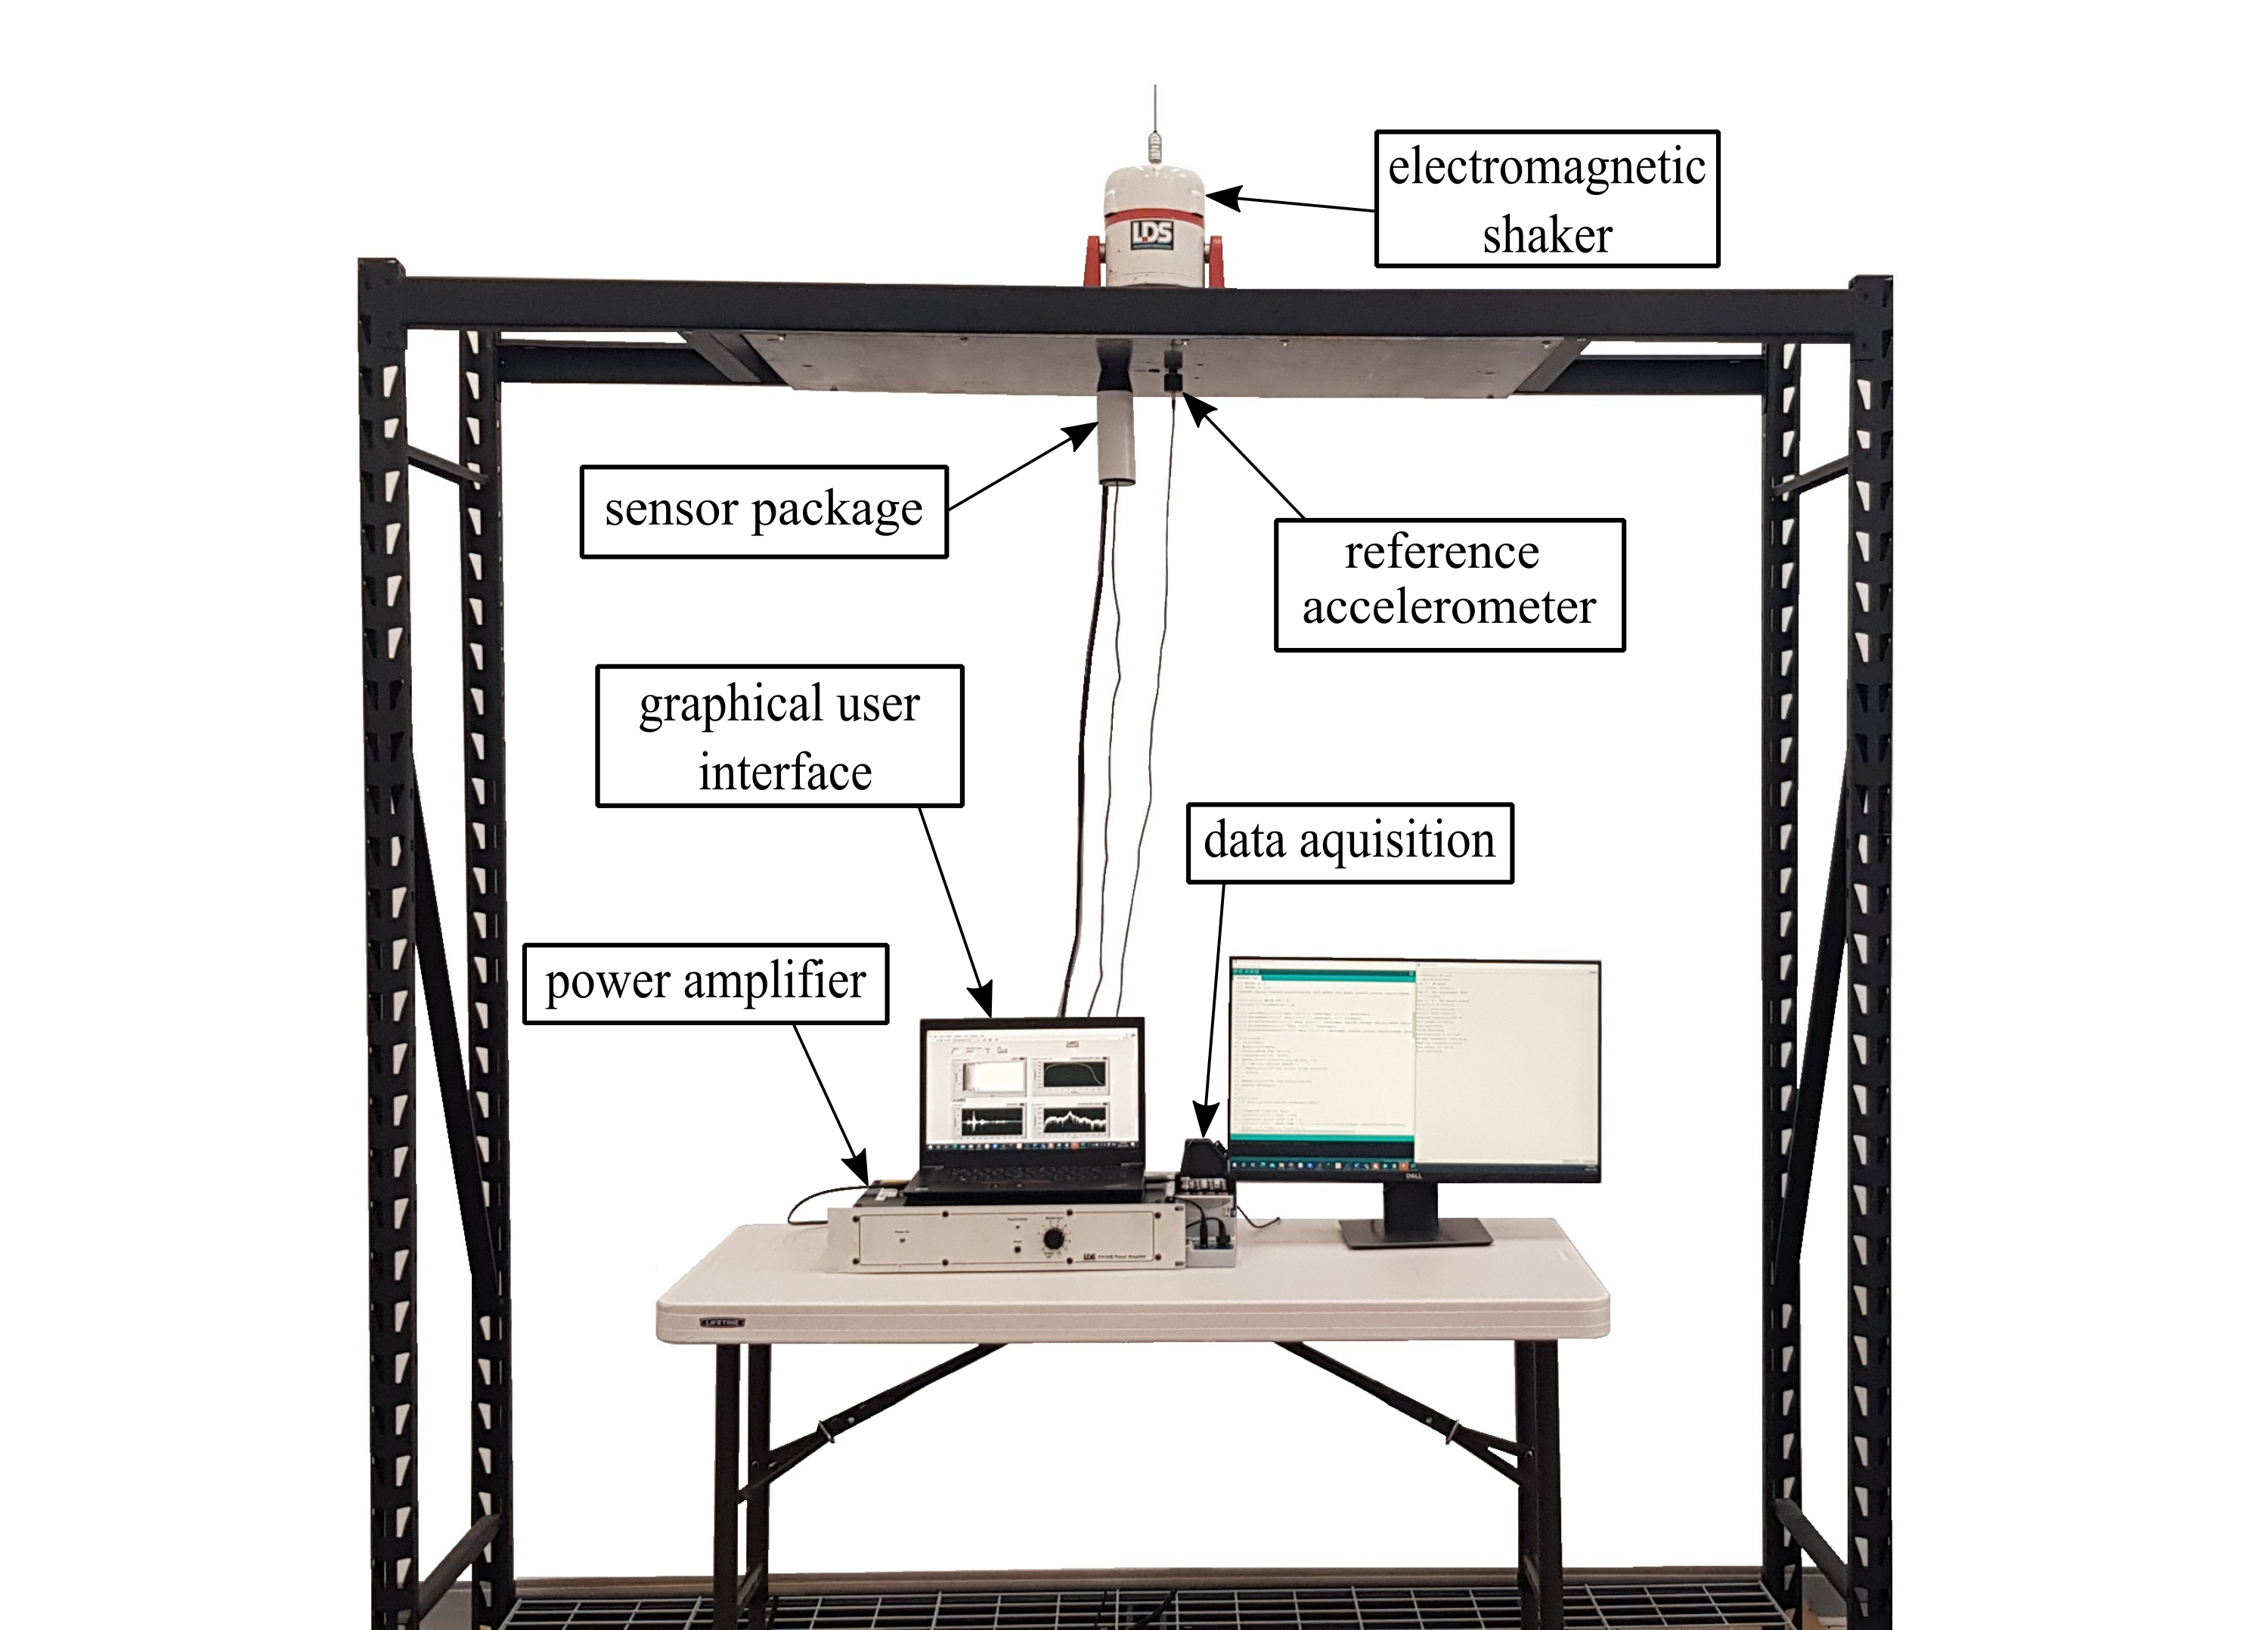
\includegraphics[width=6 in]{figures/structure experimental setup.png}
		\caption{Structure test setup with labeled key components.}
		\label{fig:structure experimental setup} 
	\end{figure}


	
	In the validation stage, a steel test structure was constructed with a data acquisition system capable of triggering both the sensor package and reference accelerometer simultaneously, generating an excitation signal to be routed to the electromagnetic shaker, and finally recording reference acceleration for later processing. The experiments were conducted using the test apparatus shown in figure~\ref{fig:structure experimental setup}. Both the reference accelerometer and sensor package were hard wired to the data acquisition trigger to ensure minimal latency when triggering. Chirp driven excitation was used to examine the filter’s performance with the same input used in the modeling process. By investigating the same input excitation, with and without a test structure, a true metric of the filter’s performance can be determined.  
		
	\section{RESULTS AND DISCUSSIONS}
	Using the data gathered from the bench top and test structure experiments, the filter was implemented using MATLAB’s system identification toolbox \cite{MAT2014}. With the inverse plant transfer function determined, the raw sensor package, filtered signal, in addition to the reference acceleration were examined. As shown in figure~\ref{fig:Chrip Structure Test}, the time domain plot indicates that the filtered signal tracing the reference with high correlation, additionally, in the frequency domain, its shown that the filter enhances the signal in the range of 6-20 Hz. When investigating error percentage as shown in figure~\ref{fig:chirp structure error}, its shown that error is considered negligible between 6-14 Hz ($<$0.4\%). Moreover, when the signal to noise ratio of the time domain signal is obtained, it is found that an increase of 1.2 dB was established, a 7.17\% enhancement from the raw sensor package data. Diminishing returns of the filter can be observed in the range below 5 Hz, where it is speculated that the analog to digital converter (ADC) onboard the sensor package’s accelerometer does not have the adequate resolution to detect the low-energy signal found in lower frequencies.
	
	\subsection{Chrip excitation structure test outcomes:}
	
	\begin{figure} [H]
		\centering
		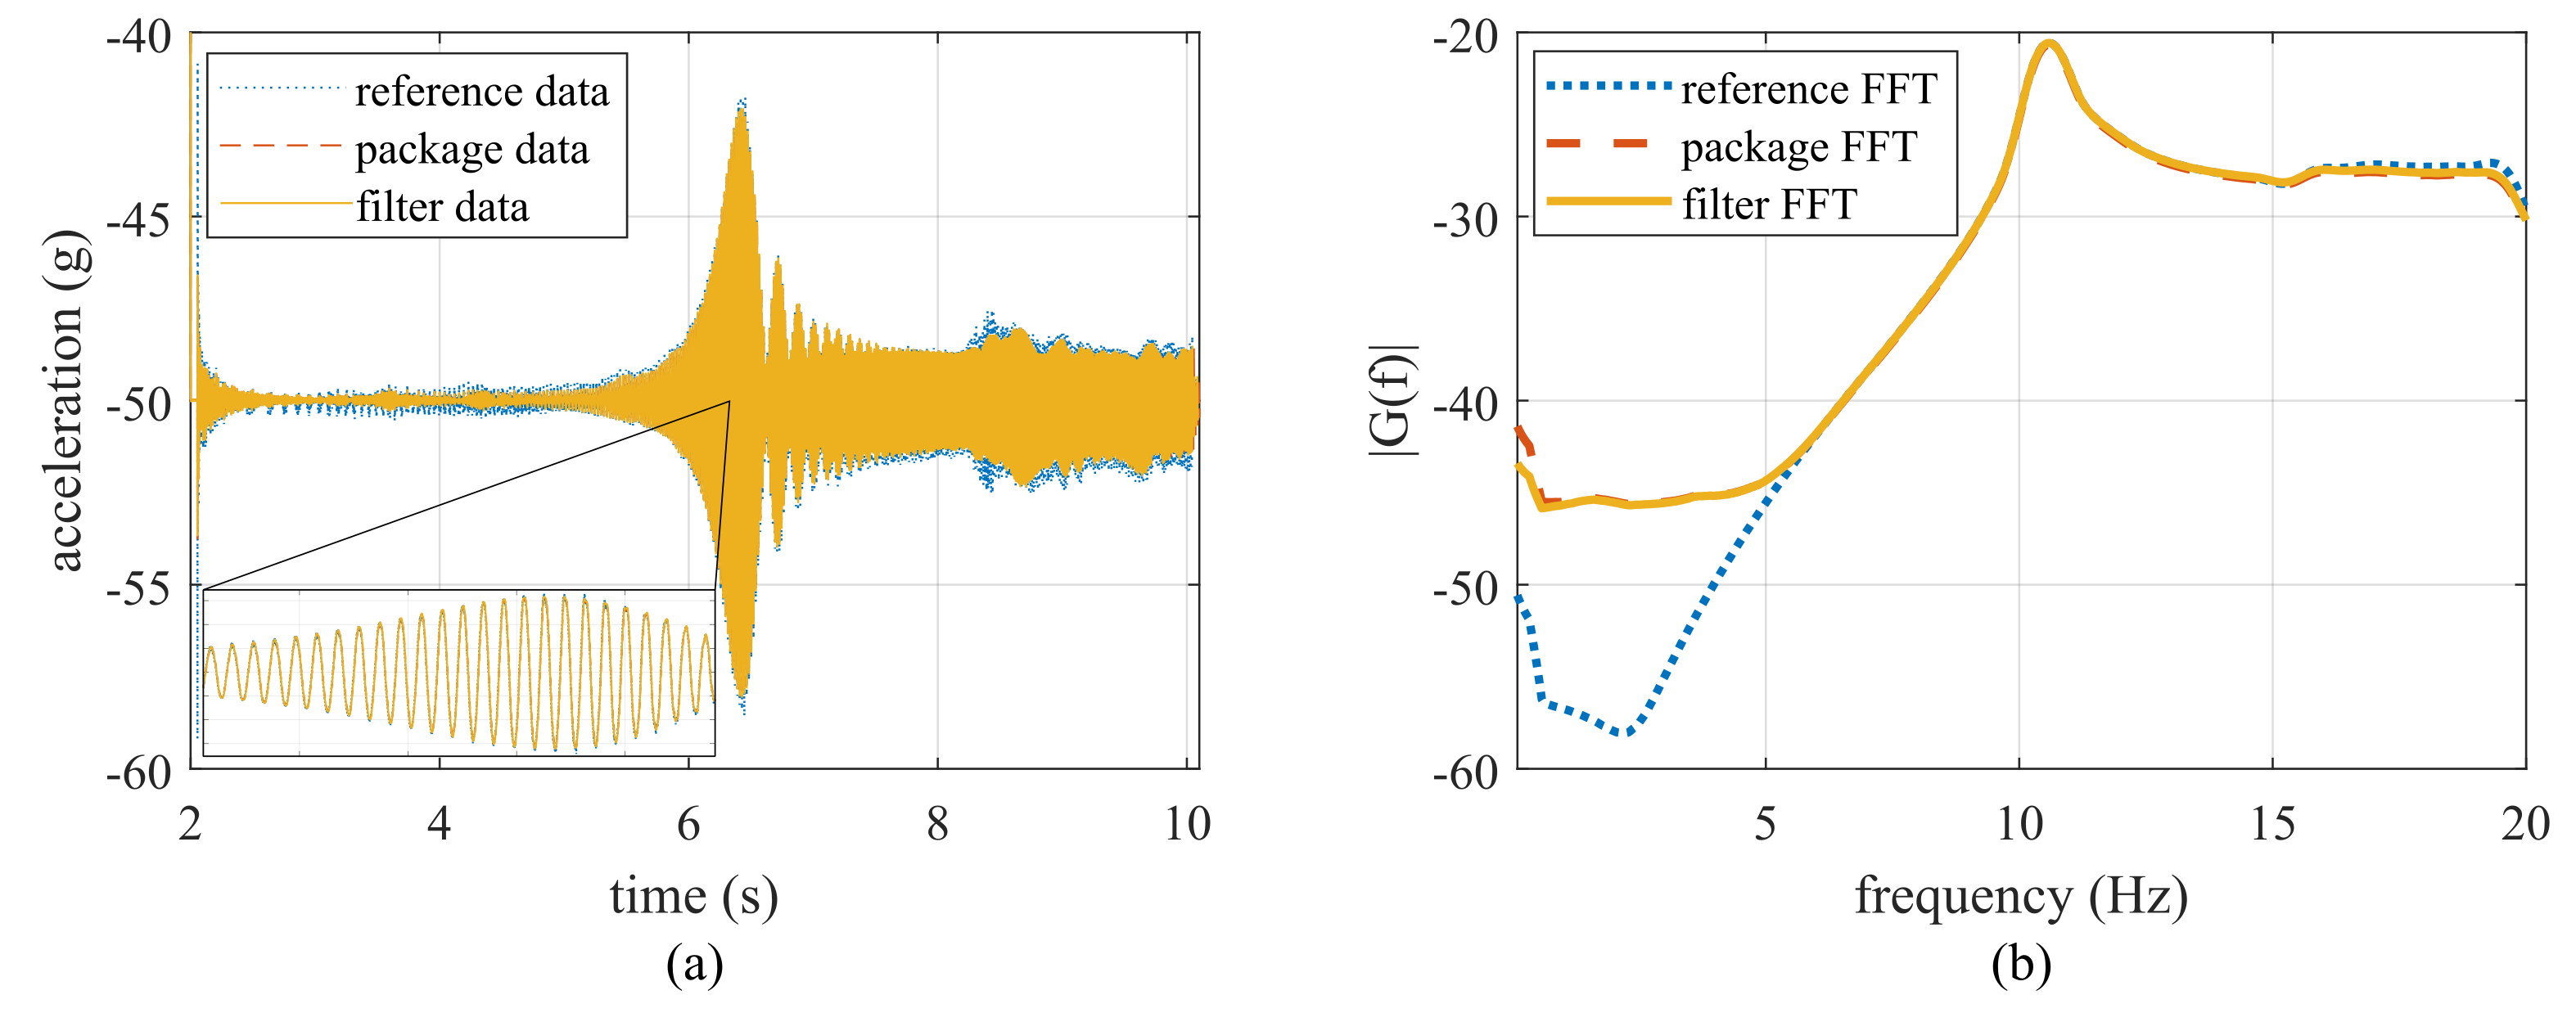
\includegraphics[width=6 in]{figures/Chrip Structure Test.png}
		\caption{Structure test comparison between pre and post filter performance in: (a) time domain; (b) frequency domain with respect to a reference accelerometer.}
		\label{fig:Chrip Structure Test} 
	\end{figure} 
	
	\begin{figure} [H]
		\centering
		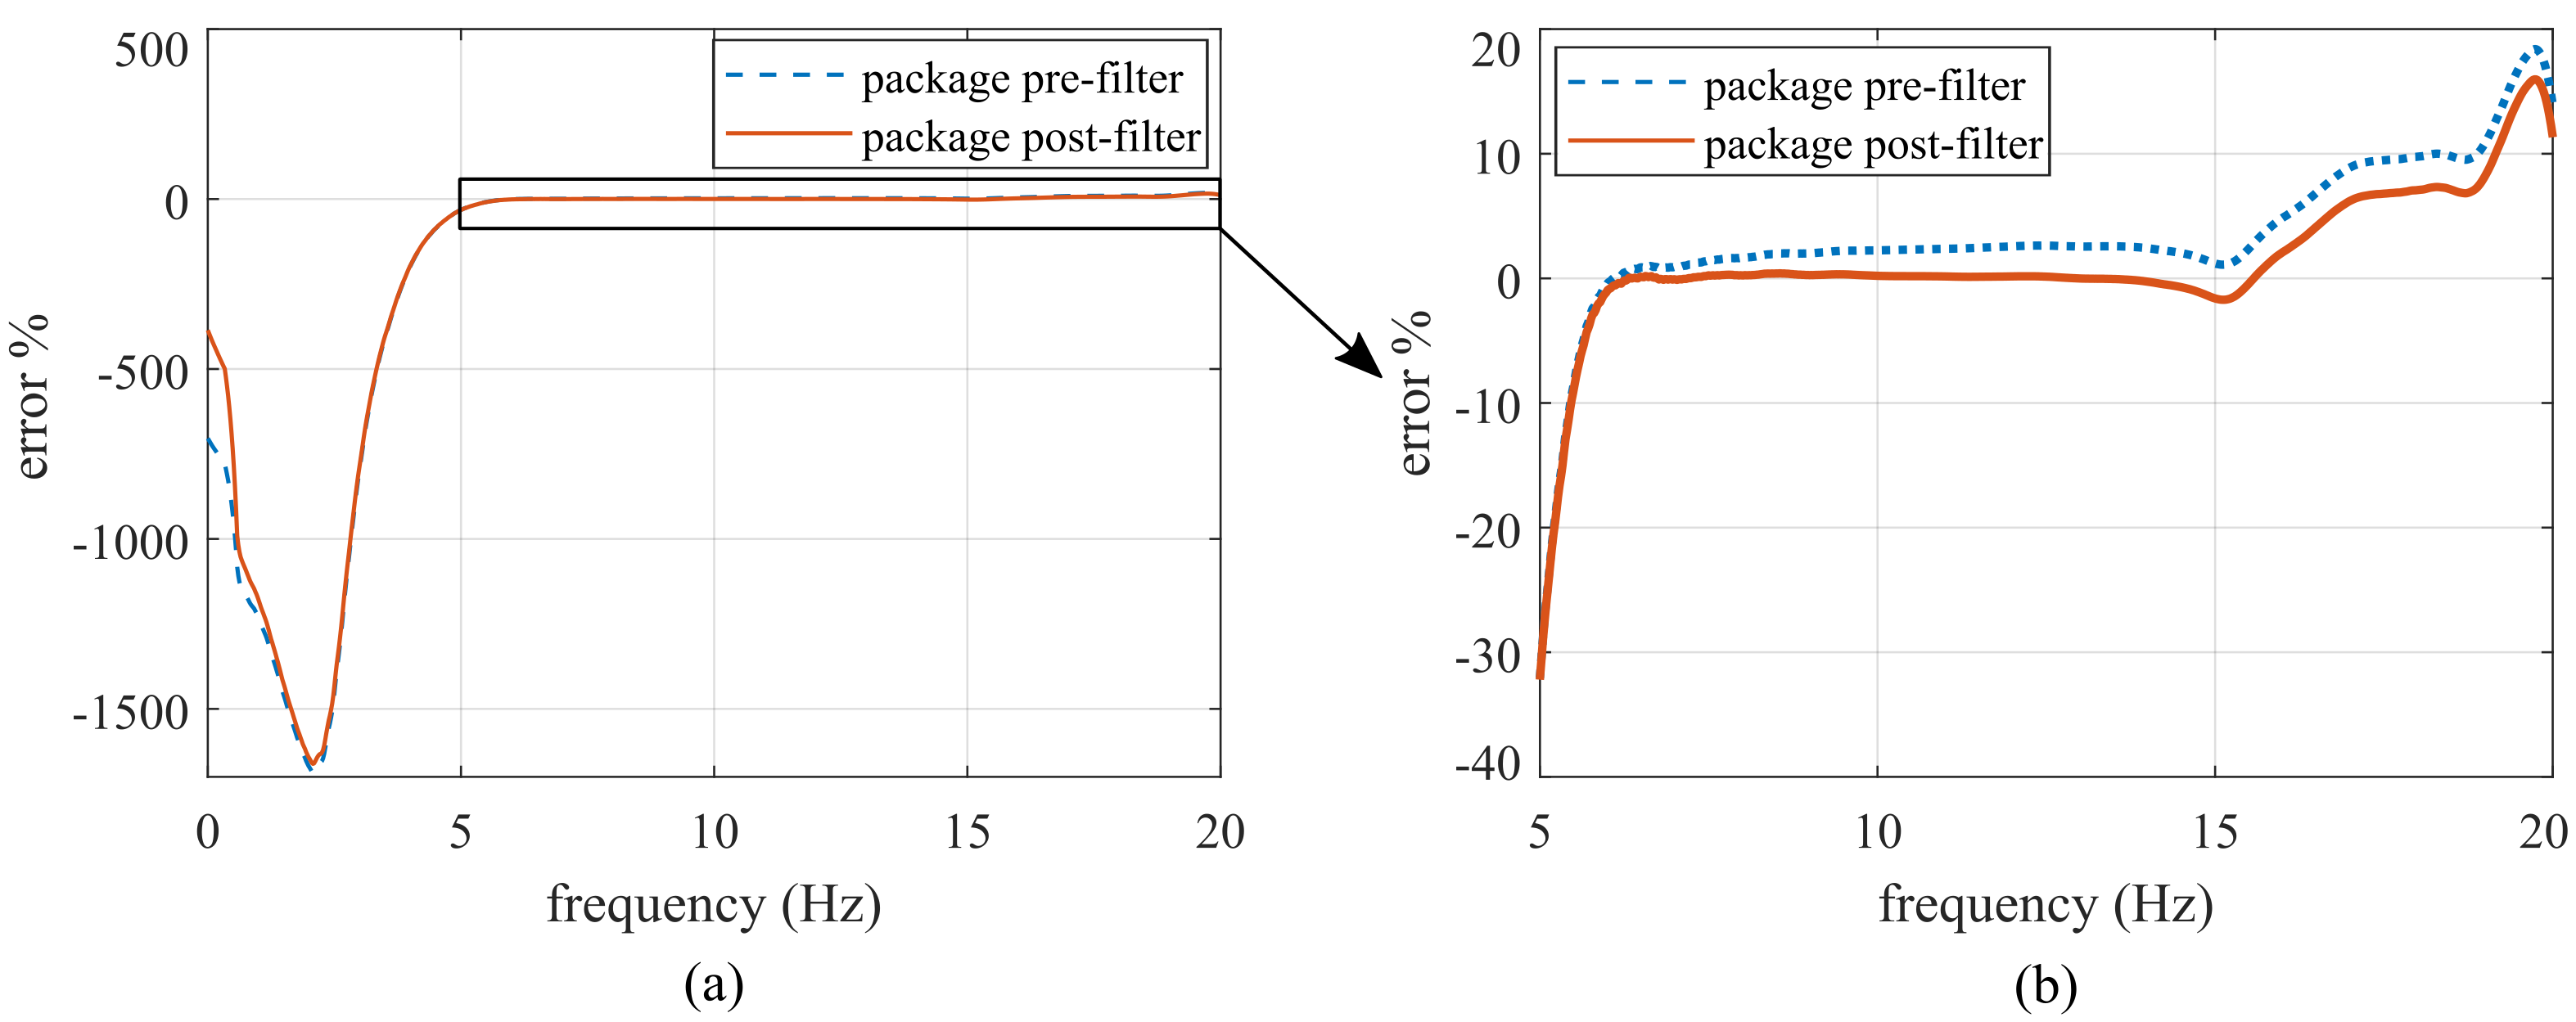
\includegraphics[height=6cm]{figures/Chirp Structure Error.png}
		\caption{Pre and post filtering frequency domain error percentage.}
		\label{fig:chirp structure error} 	
	\end{figure} 

	\begin{table}[H]
	\caption{Signal to noise ration report of the chirp-based filter applied to the test structure’s data.} 
	\label{tab:SNR Report}
	\begin{center}       
		\begin{tabular}{|c|c|c|} 
			\hline
			\rule[-1ex]{0pt}{3.5ex}  Pre-filter SNR & 16.74 dB & - \\
			\hline
			\rule[-1ex]{0pt}{3.5ex}  Post-filter SNR & 17.94 dB & - \\
			\hline
			\rule[-1ex]{0pt}{3.5ex}  SNR increase & 1.2 dB & 7.17\% \\
			\hline
		\end{tabular}
	\end{center}
	\end{table}
	
	\section{CONCLUSION}
	In this work, the design of a low-cost high mobility structural health monitoring system was presented. From sensor package design and testing to the UAV delivery and retrieval experiments, along with wireless capabilities. A frequency response filter was implemented to compensate for the loss of transmissibility between the structure and the accelerometer, caused by the sensor package. Experimental results demonstrated that the filter provided a 7.17\% enhancement over the raw sensor package data with significant improvement is the accuracy of the sensor package between 6 and 15 Hz. The performance limitation seen in the range below 5 Hz is attributed to multiple factors including short comings in the analog to digital resolution, noise bed level, the challenges accompanied with modeling low-energy signals. Future work on this system will include further improvement on the accelerometer signal conditioning and extending the ADC resolution to meet the required threshold.  
	
	\acknowledgments % equivalent to \section*{ACKNOWLEDGMENTS}       
	
	This material is based upon work supported by the University of South Carolina through grant number 80004440. Any opinions, findings, and conclusions or recommendations expressed in this material are those of the authors and do not necessarily reflect the views of the University of South Carolina.

	% References
	\bibliography{ReferancesReport} % bibliography data in report.bib
	\bibliographystyle{spiebib} % makes bibtex use spiebib.bst
	
\end{document} 